\documentclass[openright,twoside,10pt]{book}
\usepackage[b5paper,left=2cm,top=2.5cm,right=1.5cm,bottom=2.5cm]{geometry} 
\usepackage[spanish, es-tabla]{babel} % espanol
\usepackage[utf8]{inputenc} % acentos sin codigo
\usepackage{graphicx} % gráficos
\usepackage{lscape}
\usepackage{fancyvrb}
\usepackage{fancyhdr}
\usepackage{wrapfig}
\usepackage[hidelinks]{hyperref}
\usepackage{biblatex}
\bibliography{bibliografia}
\usepackage{float}
\usepackage{libertine}

\providecommand{\tightlist}{%
  \setlength{\itemsep}{0pt}\setlength{\parskip}{0pt}}
  
\setlength{\parskip}{10pt plus 1pt minus 1pt}
 % aqui definimos el encabezado de las paginas pares e impares.
\rhead[]{}

\renewcommand{\headrulewidth}{0.5pt}

% aqui definimos el pie de pagina de las paginas pares e impares.
\rfoot[\thepage]{\thepage}
\cfoot[]{}
\renewcommand{\footrulewidth}{0pt}

%redefino el verbatim
%\renewenvironment{verbatim}{\begin{Verbatim}[frame=single,fontsize=\small]}{\end{Verbatim}}


% aqui definimos el encabezado y pie de pagina de la pagina inicial de un capitulo.
\fancypagestyle{plain}{
\fancyhead[R]{}
\fancyfoot[C]{}
\fancyfoot[R]{\thepage}
\renewcommand{\headrulewidth}{0.5pt}
\renewcommand{\footrulewidth}{0pt}
}

\pagestyle{fancy} % seleccionamos un estilo

\date{22 de junio de 2017}
\author{Julio Gracia Gutiérrez}
\title{Desarrollo de software educativo de apoyo a la docencia en la teoría de
conjuntos.}

\begin{document}
    {
        \fontfamily{phv}\selectfont
        \begin{titlepage}
        \begin{center}
            \vspace*{-1in}
            \begin{figure}[htb]
                \begin{center}
                    
\includegraphics[width=3cm]{./latex/img/logo}
                \end{center}
            \end{figure}
            \begin{Large}
                \textbf{Universidad de Valladolid}
            \end{Large}

            \vspace*{0.15in}
            \vspace*{0.6in}
            \begin{Huge}
                {Escuela de Ingeniería Informática\\}
            \end{Huge}
            \vspace*{0.2in}
            \begin{Large}
                \textbf{\textsc{Trabajo Fin de Grado\\}}
            \end{Large}
            \vspace*{0.5in}
            \begin{Large}
                { Grado en Ingeniería Informática}\\
                { Mención en INGENIERÍA DE SOFTWARE \\}
            \end{Large}
            \vspace*{0.5in}
            %\rule{140mm}{0.1mm}\\
            \vspace*{0.3in}
            \begin{large}
                \textbf{{\LARGE Desarrollo de software educativo de apoyo a la docencia en la teoría de
conjuntos.\\}}
            \end{large}
            \vspace*{0.3in}
            %\rule{140mm}{0.1mm}\\
            \vspace*{1.3in}
            \begin{large}
                \begin{flushright}
                    Autor:\\
                    \textbf{Julio Gracia Gutiérrez} \\
                    \vspace*{0.3in}
                    Tutor:\\
                    \textbf{María Felisa Pérez Martínez}
                \end{flushright}
            \end{large}
        \end{center}
    \end{titlepage}

    }
    
    \newpage
    \mbox{}	
    \thispagestyle{empty} % para que no se numere esta página

    \chapter*{}
    \pagenumbering{Roman} % para comenzar la numeración de paginas en números romanos

    \begin{flushright}
        \textit{%Dedicatoria,\\
        Dedicatoria ejemplo}
    \end{flushright}

    \chapter*{Agradecimientos} % si no queremos que añada la palabra "Capitulo"
    \addcontentsline{toc}{chapter}{Agradecimientos} % si queremos que aparezca en el índice
    \markboth{AGRADECIMIENTOS}{AGRADECIMIENTOS} % encabezado 

    Agradecimiento ejemplo

    \chapter*{Resumen} % si no queremos que añada la palabra "Capitulo"
    \addcontentsline{toc}{chapter}{Resumen} % si queremos que aparezca en el índice
    \markboth{RESUMEN}{RESUMEN} % encabezado
    %\begin{flushleft}

    En el presente trabajo se va a desarrollar un software de ayuda para la
    asignatura ``Matemática Discreta''. El objetivo del presente TFG es
    desarrollar un prototipo funcional de una aplicación web orientada a
    mejorar el aprendizaje y el afianzamiento de los conceptos relativos a
    la asignatura. En este punto será necesario plantear la arquitectura de
    la aplicación que se va a implementar.
    
    La solución escogida consiste en utilizar Angular programado en
    TypeScript para el front-end, Node.js programado en JavaScript y una
    base de datos relacional MariaDB para el back-end. Angular es una
    plataforma de desarrollo para aplicaciones web de TypeScript de código
    abierto. Node.js es un entorno en tiempo de ejecución multiplataforma
    asíncrono, de código abierto, para la capa del servidor. MariaDB es un
    sistema de gestión de bases de datos derivado de MySQL.
    
    Palabras clave: Angular, Node.js, MariaDB, código abierto, TypeScript,
    JavaScript.

    %\end{flushleft}


    \chapter*{Abstract} % si no queremos que añada la palabra "Capitulo"
    \addcontentsline{toc}{chapter}{Abstract} % si queremos que aparezca en el índice
    \markboth{ABSTRACT}{ABSTRACT} % encabezado
    \begin{flushleft}

    Traducción

    \end{flushleft}

    \tableofcontents % indice de contenidos

    \cleardoublepage
    \addcontentsline{toc}{chapter}{Lista de figuras} % para que aparezca en el indice de contenidos
    \listoffigures % indice de figuras

    \cleardoublepage
    \addcontentsline{toc}{chapter}{Lista de tablas} % para que aparezca en el indice de contenidos
    \listoftables % indice de tablas

    \chapter{Introducción}
    
    \section{Descripción del problema}\label{descripciuxf3n-del-problema}
    
    \pagenumbering{arabic}
    
    Los alumnos que entran en el primer curso de una ingeniería experimentan
    unos grandes cambios a nivel académico. Esto es debido a que cambia la
    metodología en la docencia y al aumento del volumen de contenidos tanto
    teóricos como prácticos en comparación con etapas anteriores. Algunas
    asignaturas se fundamentan en los conocimientos adquiridos durante los
    cursos de bachillerato pero otras tienen contenidos totalmente nuevos.
    La procedencia de los estudiantes es heterogénea: PAU y Módulos
    Superiores y ,por tanto, habrán tenido diferente grado de contacto con
    los contenidos de la titulación. En particular, Matemática Discreta
    incluye conceptos y resultados matemáticos que no han sido explorados
    con anterioridad. Esta asignatura forma parte de las asignaturas de
    carácter básico.
    
    Para tener una buena base en informática es necesario conseguir un buena
    base matemática teórica. En el primer año del grado, los estudiantes
    pueden experimentar una falta de motivación en asignaturas de este tipo
    debido a la complejidad de las mismas y a que no consiguen encontrar una
    aplicación práctica real ni son conscientes de su importancia, tanto
    para asignaturas futuras como para su vida profesional.
    
    Con la asiganatura Matemática Discreta se pretende ofrecer una formación
    básica y sólida al futuro ingeniero informático. Básica, en el sentido
    que los diferentes aspectos serán tratados a un nivel introductorio, y
    sólida, en el sentido de que los conocimientos adquiridos deben sentar
    las bases para desenvolverse en el resto de su formación académica y
    desarrollo profesional. Se trata de habilitar a los estudiantes para que
    adquieran las destrezas necesarias para seguir aprendiendo a lo largo de
    la vida los aspectos de la Informática relacionados con la lógica,
    teoría de conjuntos y combinatoria, como son la inteligencia artificial,
    el uso de bases de datos o la estadística.
    
    El presente trabajo se va a centrar en mejorar el aprendizaje y la
    resolución de dudas respecto a la asignatura.
    
    \section{Objetivo}\label{objetivo}
    
    El objetivo final de este trabajo es mejorar el estudio de la
    asignatura, facilitando el afianzamiento de los conocimientos. Para
    ello, se busca crear una plataforma que facilite la comunicación
    alumno-profesor, y dote al profesor de las herramientas para facilitar
    la distribución de los contenidos de la asignatura, así como permitiendo
    al alumno comprobar sus conocimientos mediante la implementación de
    tests. En definitiva, se busca mejorar la preparación de los alumno para
    afrontar la asignatura satisfactoriamente, ya que esta sienta unas bases
    muy importantes para otras de cursos futuros.
    
    \section{\texorpdfstring{Contexto
    \cite{guiamatematicadiscreta}}{Contexto }}\label{contexto}
    
    La metodología docente actual de la asignatura se basa en la combinación
    de sesiones teórico-prácticas en aula, sesiones prácticas en grupos
    reducidos y trabajo, tanto grupal como individual. Concretamente se
    destinan 28 horas a las clases teórico-prácticas, 30 horas a las
    prácticas, 10 horas al estudio y trabajo grupal y 80 horas al estudio y
    trabajo individual. El presente trabajo se centra en este último
    apartado, ya que considero que es en el que el alumno puede sufrir
    mayores dificultades, al no contar con la dirección del profesor ni con
    la ayuda de un grupo.
    
    El desarrollo de la asignatura consiste en clases magistrales
    participativas, en las que se imparten conocimientos que deben ser
    asimilados con las horas de estudio individual. Gracias al afianzamiento
    de los conocimientos, el alumno será capaz de participar de forma activa
    en las sesiones prácticas y teóricas, así como superar
    satisfactoriamente las diversas pruebas escritas a lo largo del curso.
    Todo ello influye positivamente en la calificación.
    
    El material básico del que dispone el alumno consiste en un documento
    pdf con los contenidos teóricos y enunciados de problemas, que forman
    los conocimientos mínimos para superar la asignatura.
    
    \section{Solución adoptada}\label{soluciuxf3n-adoptada}
    
    Debido al tamaño del temario y a su complejidad, el estudio de esta
    asignatura puede resultar difícil. Tampoco ayuda el formato del material
    básico, ya que es un documento PDF que no cuenta con ningún marcador.
    Esto dificulta enormemente la búsqueda de un concepto concreto, así como
    la relación entre conceptos, ya que las unicas herramientas con la que
    los alumnos cuentan para ello son las palabras claves, que están
    resaltadas en negrita y la función de búsqueda de palabras del editor de
    PDF utilizado.
    
    Por otro lado, el procedimiento para plantear dudas requiere que el
    alumno se ponga en contacto con el profesor, ya sea presencialmente o
    mediante el correo electrónico, y el profesor resuelva la duda de manera
    individual. La duda, por tanto, será respondida únicamente a nivel
    personal, por lo que es complicado que el resto de alumnos se enteren de
    las dudas que han planteado sus compañeros y de las soluciones que el
    profesor ha dado a dichas dudas. A su vez, esto puede conllevar que el
    profesor resuelva varias veces la misma duda.
    
    Finalmente, es necesario algún sistema que permita al alumno saber de
    forma aproximada su nivel de preparación para ayudarle a afrontar las
    etapas finales de la asignatura.
    
    Lo que buscamos es una herramienta que nos permita buscar conceptos de
    forma rápida, entender las relaciones entre conceptos, reducir el tiempo
    malgastado tanto por parte del profesor como del alumno, evitando el
    planteamiento repetido de dudas ya resueltas con anterioridad y
    facilitando al alumno la resolución concreta de dudas y, por último,
    dotar al alumno de un mecanismo de comprobación de conocimientos. Esta
    herramienta debe ser accesible por cualquier miembro de la comunidad
    educativa de la Universidad de Valladolid.
    
    \section{Estructura de la memoria}\label{estructura-de-la-memoria}
    
    En base al esquema seguido para la realización del presente trabajo, se
    ha estructurado la memoria de la misma manera:
    
    PLAN DE PROYECTO: En este capítulo se detalla la planificación del
    proyecto.
    
    TECNOLOGÍAS UTILIZADAS: En este capítulo se detalla infromación sobre
    las tecnologías escogidas, así como se explican ciertos conceptos clave
    para entenderlas.
    
    DESARROLLO DEL PROYECTO: La parte fundamental del proyecto es el
    desarrollo de un prototipo de plataforma web. En este apartado se
    profundizará en el proceso de desarrollo, que incluye las etapas de
    análisis, desarrollo y despliegue.
    
    CONCLUSIONES Y RESULTADOS: Tras realizar una serie de pruebas al
    prototipo, se presentarán las conclusiones y se analizarán los
    resultados así como posibles mejoras a tener en cuenta.
    
    \chapter{ Tecnologías utilizadas }
    
    \section{Definiciones previas
    necesarias}\label{definiciones-previas-necesarias}
    
    \begin{itemize}
    \item
      \textbf{JavaScript:} \cite{mozilla_javascript} JavaScript (abreviado
      como JS) es un lenguaje multi-paradigma, ligero e interpretado.
    \item
      \textbf{TypeScript:} \cite{enriqueoriol2017, stackoverflow_Typescript}
      TypeScript es un superconjunto de JavaScript que permite el uso de
      clases, interfaces y tipado estático. El uso de variables tipadas de
      TypeScript aporta mayor robustez al código.
    \item
      \textbf{ECMAScript:} \cite{mozilla_ecmascript} ECMAScript (abreviado
      como ES) es un lenguaje de scripting que forma la base de JavaScript.
      Está recogido en los estándares ECMA-262 y ECMA-402 de ECMA
      International. Al referirnos a ES5 nos referimos a la quinta versión
      del estándar ECMA-262, mientras que al hablar de ES2015 o ES6 nos
      referimos al estándar ECMA-262 en su sexta versión. Actualmente los
      navegadores soportan ES5, por lo cualquier lenguaje derivado de
      ECMAScript(como son JavaScript y TypeScript) deben de ser traspilado a
      ES5.
    \item
      \textbf{Transpilar:}
      \cite{enriquefernandezguerra_typescript, builtbyedgar_transpilar}
      Transpilar es un término relativamente nuevo, proviene del inglés
      \emph{transpiler}, fruto de la unión de las palabras \emph{translate}
      y \emph{compiler}. Es la operación de traducción de un lenguaje a
      otro, siendo ambos del mismo nivel de abstracción aproxiamadamente.
    \item
      \textbf{Gestor de paquetes:} \cite{debian_gestorpaquetes} Un gestor de
      paquetes mantiene un registro del software que está instalado en su
      ordenador, y le permite instalar software nuevo, actualizarlo a
      versiones más recientes, o eliminar software de una manera sencilla.
      Como su propio nombre sugiere, los gestores de paquetes gestionan
      paquetes: conjuntos de ficheros que se agrupan y que puede instalar y
      eliminar como conjunto. La labor de un gestor de paquetes es la de
      presentar una interfaz que asista al usuario en la tarea de
      administrar el conjunto de paquetes que están instalados en su
      sistema.
    \item
      \textbf{Plataforma:} Una plataforma es un sistema que engloba los
      componentes, interfaces y librerías necesarios para permitir a los
      desarrolladores compilar, ejecutar y depurar sus aplicaciones.
    \item
      \textbf{Framework:} Desde el punto de vista del desarrollo de
      software, un framework es una estructura de soporte definida, en la
      cual otro proyecto de software puede ser organizado y desarrollado.
    \item
      \textbf{Open source:} \cite{opensource_definition} La terminología
      open source incluye a aquellos softwares que cumplen los siguientes
      requisitos:
    
      \begin{itemize}
      \tightlist
      \item
        \textbf{Distribución libre:}La licencia no restringirá a ninguna de
        las partes vender o regalar el software como un componente de un
        conjunto de software.
      \item
        \textbf{Código fuente:} El programa debe incluir el código fuente
        sin ofuscar o dotar de un mecanismo para conseguirlo,
        preferentemente de forma gratuita mediante una descarga online.
      \item
        \textbf{Trabajos derivados:} La licencia debe permitir
        modificaciones y trabajos derivados, y permitir que se distribuyan
        de forma libre.
      \item
        \textbf{Integridad del código fuente del autor:} La licencia podría
        permitir no distribuir el código fuente del programa modificado si
        permite la distribución de parches. La licencia debe permitir
        explícitamente la distribución del software construido a partir de
        las fuentes modificadas.
      \item
        \textbf{Sin discriminación:} La licencia no debe discriminar a
        ninguna persona ni colectivo.
      \item
        \textbf{Para todos los ámbitos:} La licencia no debe restringir el
        uso en función del ámbito para el que se vaya a utilizar el
        software.
      \item
        \textbf{Distribución de licencia:} Los derechos asociados al
        software deben aplicarse a todos los programas redistribuidos.
      \item
        \textbf{La licencia no debe estar asociada a un producto:} Los
        derechos del software no deben depender del paquete de software en
        el que se distribuya
      \item
        \textbf{La licencia no debe restringir a otros programas que se
        distribuyan junto a ella.}
      \item
        \textbf{La licencia debe ser independiente de la tecnología
        utilizada.}
      \end{itemize}
    \item
      \textbf{Back-end:} Término técnico para la capa de acceso a datos.
    \item
      \textbf{Front-end:} Término técnico para la capa de presentación de
      una aplicación. Concierne los componentes externos del sitio o
      aplicación web.
    \item
      \textbf{Propiedad:} \cite{mozilla_properties} Una propiedad de un
      objeto puede ser explicada como una variable que se adjunta al objeto.
      Las propiedades de un objeto definen las características de un objeto.
      Un valor de propiedad puede ser una función, la cual es conocida
      entonces como un método del objeto.
    \item
      \textbf{Licencia GPL:} \cite{GNU_GPL, GNU_copyleft} La licencia GPL o
      GNU GPL es una licencia copyleft. Esto es, un método general que
      requiere que todas las versiones modificadas y extendidas sean también
      libres.
    \item
      \textbf{API:} API significa interfaz de programación de aplicaciones
      (Application Programming Interface). Las APIs ofrecen una forma de
      estándar de dotar de funcionalidad a una aplicación, definiendo que
      funciones y métodos son accesibles.
    \end{itemize}
    
    \section{Node.js}\label{node.js}
    
    \begin{figure}[H]
        \begin{center}
            
\includegraphics[scale=0.05]{img/nodejs.png}
        \end{center}
        \caption{Logo de Node.js}
    \end{figure}
    
    Node.js es un entorno de ejecución para JavaScript construido con el
    motor de JavaScript V8 de Chrome
    
    \subsection{Instalación}\label{instalaciuxf3n}
    
    Para instalar node vamos a usar nvm. En este proyecto utilizaremos la
    versión \textbf{6.9.5}
    
    \begin{verbatim}
    curl -sL \
    https://raw.githubusercontent.com/creationix/nvm/v0.32.0/install.sh \
    -o install_nvm.sh
    bash install_nvm.sh
    export NVM_DIR="/root/.nvm"
    [ -s "$NVM_DIR/nvm.sh" ] && . "$NVM_DIR/nvm.sh"
    \end{verbatim}
    
    En este proyecto usaremos la versión \textbf{6.9.5}
    
    \begin{verbatim}
    nvm install v6.9.5
    \end{verbatim}
    
    \section{NPM}\label{npm}
    
    \begin{figure}[H]
        \begin{center}
            
\includegraphics[scale=0.8]{img/npm.png}
        \end{center}
        \caption{Logo de NPM}
    \end{figure}
    
    Npm es un gestor de paquetes que permite a los desarrolladores de
    JavaScript compartir y reutilizar código. Gracias a este gestor podemos
    conseguir de forma sencilla y actualizada las dependencias que va a
    tener nuestra aplicación. Este gestor de paquetes resulta esencial, ya
    que de él dependen Angular, Angular CLI y Node.js.
    
    \subsection{Instalación:}\label{instalaciuxf3n-1}
    
    NPM es instalado junto con Node.js en el apartado anterior. Vamos a
    actualizarlo.
    
    \begin{verbatim}
    npm install -g npm
    \end{verbatim}
    
    \subsection{Principales comandos
    utilizados:}\label{principales-comandos-utilizados}
    
    \begin{itemize}
    \item
      \texttt{npm\ install}
    
      Este comando instala todas las dependencias que hayamos declarado en
      nuestro fichero de configuración.En caso de especificar un nombre al
      final del comando instalaremos únicamente la dependencia nombrada.
      Este comando instala los paquetes elegidos, así como todos los
      paquetes de los que estos dependa. Usualmente se usará la opción
      --save que nos guarda la dependencia en nuestro fichero de
      configuración, de forma que podamos instalarla posteriormente
    \item
      \texttt{npm\ uninstall\ {[}nombre{]}}
    
      Este comando elimina la dependencia nombrada de nuestro sistema.
      Usualmente, se usará la opción --save para eliminarla también del
      fichero de configuración.
    \end{itemize}
    
    \section{Express}\label{express}
    
    \begin{figure}[H]
        \begin{center}
            
\includegraphics[scale=0.3]{img/express.png}
        \end{center}
        \caption{Logo de Express}
    \end{figure}
    
    Express es un framework de desarrollo de aplicaciones web y APIs para
    Node.js
    
    \subsection{Instalación}\label{instalaciuxf3n-2}
    
    \begin{verbatim}
    npm install express
    \end{verbatim}
    
    \subsection{Principales utilidades}\label{principales-utilidades}
    
    Nos facilita el manejo de:
    
    \begin{itemize}
    \tightlist
    \item
      \textbf{Estáticos:} Ruta pública donde generalmente se alojan assets
      (CSS, imágenes, JS).
    \end{itemize}
    
    \begin{verbatim}
    app.use(express.static(path.join(__dirname, 'public')));
    \end{verbatim}
    
    \begin{itemize}
    \tightlist
    \item
      \textbf{Controladores:} Encargados de controlar las peticiones http.
    \end{itemize}
    
    \begin{verbatim}
    app.post('/login', function(req, res) {});
    \end{verbatim}
    
    \begin{itemize}
    \tightlist
    \item
      \textbf{Sesiones y cookies:}
    \end{itemize}
    
    \begin{verbatim}
    app.use(express.cookieParser('your secret here'));
    app.use(express.session());
    \end{verbatim}
    
    \section{\texorpdfstring{Angular
    \cite{angular_docs}}{Angular }}\label{angular}
    
    \begin{figure}[H]
        \begin{center}
            
\includegraphics[scale=0.6]{img/angular.png}
        \end{center}
        \caption{Logo de angular}
    \end{figure}
    
    Angular es una plataforma open source de desarrollo de front-end
    desarrollado por Google. Está basado en componentes, que es una
    combinación de una plantilla HTML con un controlador.
    
    Si bien está desarrollado con Javascript y permite el desarrollo con ES5
    o superior, la comunidad de desarrolladores(incluyendo los responsables
    del proyecto de Google) prefiere utilizar TypeScript.
    
    \begin{figure}[H]
        \begin{center}
            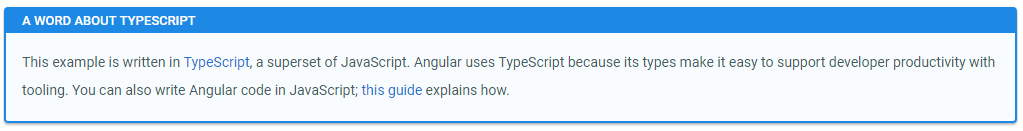
\includegraphics[width=\textwidth]{img/aboutTypescript.png}
        \end{center}
        \caption{Google sobre TypeScript}
    \end{figure}
    
    \subsection{¿Qué es un controlador?}\label{quuxe9-es-un-controlador}
    
    \begin{verbatim}
    @Component({
        selector: ‘my-app’,
        template: <h1>Hello {{name}}</h1>
    })
    \end{verbatim}
    
    Todos los componentes inician con el decorador \textcite{Component} que
    describe cómo se comporta el componente. Entre otras opciones, define
    como incluir el componente en una página HTML, mediante la propiedad
    selector; y como está estructurado visualmente mediante la propiedad
    template. En el ejemplo dado, si quisiéramos utilizar el componente en
    una página HTML se usaría el elemento
    \texttt{\textless{}my-app\textgreater{}}, y el componente se ve como la
    frase ``Hello \{\{name\}\}'' dentro de un elemento de de título 1.
    
    En un desarrollo de mayor tamaño en lugar de definir la plantilla HTML
    en el propio componente, se usará la propiedad \texttt{templateUrl} para
    definir dónde buscar la plantilla HTML. De igual forma, se separarían
    los códigos CSS mediante la propiedad \texttt{styleUrls}. Ejemplo:
    
    \begin{verbatim}
    @Component({
        selector: ‘my-app’,    
        templateUrl: 'nombre_del_archivo.html',
        styleUrls: ['nombre_del_archivo1.css', 'nombre_del_archivo2.css']
    })
    \end{verbatim}
    
    Siguiendo la trayectoria de AngularJs, precursor del actual Angular,
    conseguimos acceder a las propiedades del controlador mediante el uso de
    \{\{ nombre\_variable \}\}. En este caso accederíamos a la propiedad
    \texttt{name}.
    
    \begin{verbatim}
    export class AppComponent { name = ‘Angular’; }
    \end{verbatim}
    
    Define la clase del controlador. En el caso de ejemplo, el controlador
    solo tiene la propiedad name, que contiene la cadena de texto
    ``Angular''
    
    \section{\texorpdfstring{Angular CLI
    \cite{angular_cli}}{Angular CLI }}\label{angular-cli}
    
    \begin{figure}[H]
        \begin{center}
            
\includegraphics[scale=0.3]{img/angular-cli.png}
        \end{center}
        \caption{Logo de angular-cli}
    \end{figure}
    
    Angular CLI es una herramienta utilizada para inicializar aplicaciones
    Angular, desarrollar componentes y para tareas de mantenimiento
    asociadas a ello.
    
    \subsection{Instalacion:}\label{instalacion}
    
    \begin{verbatim}
    npm install -g @angular/cli
    \end{verbatim}
    
    \subsection{Comandos relevantes
    utilizados:}\label{comandos-relevantes-utilizados}
    
    \begin{itemize}
    \item
      \texttt{ng\ new\ {[}nombre{]}}
    
      Inicializa una nueva aplicación Angular con el nombre elegido.
    \item
      \texttt{ng\ serve}
    
      Transpila la aplicación y monta un servidor web.
    \item
      \texttt{ng\ generate\ class\ {[}nombre{]}}
    
      Genera una clase con el nombre escogido. Una clase es una construcción
      que permite crear tipos personalizados mediante la agrupación de
      variables de otras clases y comportamientos comunes.
    \item
      \texttt{ng\ generate\ component\ {[}nombre{]}}
    
      Genera un componente con el nombre escogido.
    \item
      \texttt{ng\ generate\ service\ {[}nombre{]}}
    
      Genera un servicio con el nombre escogido. Un servicio es una función,
      con sus propiedades y métodos que puede ser incluida, mediante
      inyección de dependencias, en los componentes. Gracias a esto, se
      pueden desarrollar funciones para tareas específicas, como es la
      comunicación con el servidor. Permite reutilizar las funciones de
      forma rápida entre componentes, así como acceder a variables
      compartidas entre ellos.
    \end{itemize}
    
    \section{Bootstrap 4}\label{bootstrap-4}
    
    \begin{figure}[H]
        \begin{center}
            
\includegraphics[scale=0.15]{img/bootstrap4.png}
        \end{center}
        \caption{Logo de Bootstrap 4}
    \end{figure}
    
    Bootstrap es un framework de HTML, CSS y JavaScript para el desarrollo
    de front-end. En su versión 4 incluye componentes de angular que
    utilizaremos en el presente proyecto.
    
    \subsection{Instalación}\label{instalaciuxf3n-3}
    
    \texttt{npm\ install\ bootstrap@4.0.0-alpha.6}
    
    \section{MariaDB}\label{mariadb}
    
    \begin{figure}[H]
        \begin{center}
            
\includegraphics[scale=0.75]{img/mariadb.png}
        \end{center}
        \caption{Logo de MariaDB}
    \end{figure}
    
    MariaDB es un sistema de gestión de bases de datos derivado de MySQL con
    licencia GPL (General Public License). Está desarrollado por Michael
    Widenius (fundador de MySQL) y la comunidad de desarrolladores de
    software libre. Surgío a partir de la compra de Sun Microsystems por
    parte de Oracle para asegurar la existencia de una versión de MySQL con
    licencia GPL.
    
    \subsection{Instalación}\label{instalaciuxf3n-4}
    
    \begin{verbatim}
    sudo apt-get install software-properties-common
    sudo apt-key adv --recv-keys --keyserver \
    keyserver.ubuntu.com 0xF1656F24C74CD1D8
    sudo add-apt-repository 'deb [arch=amd64] \
    http://tedeco.fi.upm.es/mirror/mariadb/repo/10.2/debian stretch main'
    sudo apt-get update
    sudo apt-get install mariadb-server
    \end{verbatim}
    
    \subsection{\texorpdfstring{Ventajas de MariaDB frente MySQL
    \cite{zeokat_mariadb, andergonzalez_mariadb, alidavergara_mariadb}}{Ventajas de MariaDB frente MySQL }}\label{ventajas-de-mariadb-frente-mysql}
    
    \begin{itemize}
    \item
      \textbf{Nuevos motores de almacenamiento más eficientes:}
    
      Aria y XtraDB vienen a reemplazar a MyISAM e InnoDB respectivamente.
      Cabe destacar el mayor rendimiento de Aria, cuando recibe consultas
      complejas y tiene que realizar tablas temporales, éstas se cachean en
      memoria en vez de escribirlas en disco.
    \item
      \textbf{Estadísticas para índices y tablas:}
    
      Esto puede ayudar para la optimización de la base de datos. Se añaden
      nuevas tablas de sistema para recoger esta información.
    \item
      \textbf{Mejoras en el rendimiento y la eficiencia con respecto a
      MySQL:}
    
      Un ejemplo de esto es la eliminación o mejora de algunas conversiones
      no necesarias respecto a los juegos de caracteres.
    \item
      \textbf{Software libre:}
    
      MariaDB está respaldada por la comunidad de software libre.
    \end{itemize}
    
    \subsection{Desventajas de MariaDB frente
    MySQL}\label{desventajas-de-mariadb-frente-mysql}
    
    \begin{itemize}
    \item
      \textbf{Coste migratorio:}
    
      En líneas generales, MySQL está más extendido, por lo que utilizar
      MariaDB suele acarrear un coste migratorio de los datos. Sin embargo,
      MariaDB asegura tener total compatibilidad. En este proyecto no nos
      afectará en absoluto.
    \end{itemize}
    
    \chapter{ Plan del proyecto }
    
    El plan de desarrollo software es el documento que dirige la gestión de
    un proyecto soft- ware. Define las funciones técnicas y de gestión de
    proyectos, actividades y tareas necesarias para satisfacer los
    requisitos del proyecto. La finalidad de esta sección es conocer los
    puntos básicos de los que consta el proyecto, proporcionar los
    fundamentos en los que se basa y transmitir los aspectos básicos tal y
    como han sido entendidos y formulados. A continuación se describirá la
    visión general del proyecto, que proporciona una descrip- ción de
    propósito, alcance y objetivos; la gestión de los procesos que explica
    el coste estimado; y la planificación las fases principales e hitos del
    proyecto.
    
    \section{Vision general}\label{vision-general}
    
    \subsection{Propósito, alcance y
    objetivos}\label{propuxf3sito-alcance-y-objetivos}
    
    El objetivo del presente proyecto es desarrollar un prototipo de
    aplicación que sirva de apoyo para la asignatura de Matemática Discreta.
    La aplicación será un complemento educativo que permitirá al alumno
    repasar los conceptos teóricos más importantes, evaluar sus
    conocimientos mediante unos cuestionarios de tipo test y realizar
    consultas al profesor. Por parte del profesor permitirá introducir
    contenidos teóricos, resolver dudas, plantear preguntas para formar los
    cuestionarios y monitorizar el desempeño de los alumnos en la misma.
    
    Toda esta información aparecerá de manera detallada en el apartado
    Análisis de Requisitos
    
    \subsection{Metodología utilizada}\label{metodologuxeda-utilizada}
    
    Explicacion --\textgreater{} Kanban?
    
    \subsection{Evolución del plan}\label{evoluciuxf3n-del-plan}
    
    El presente documento se revisará a lo largo del Trabajo de Fin de
    Grado, y se irá actualizando conforme a los cambios que surjan.
    
    \section{Gestión del proceso}\label{gestiuxf3n-del-proceso}
    
    \subsection{Estimación}\label{estimaciuxf3n}
    
    Se considerará que la dedicación media al proyecto será de un total de 6
    horas diarias con un solo recurso, con un día semanal de descanso.
    
    \subsection{Plan de trabajo}\label{plan-de-trabajo}
    
    \begin{itemize}
    \tightlist
    \item
      \textbf{Reunión con el cliente y documentación}
    
      \begin{itemize}
      \tightlist
      \item
        Recopilar información sobre el objetivo que persigue el cliente
        mediante entrevistas personalizadas, así como estudio de la
        documentación que este nos facilite.
      \item
        \textbf{Duración:} 1 semana
      \end{itemize}
    \item
      \textbf{Elicitación de requisitos}
    
      \begin{itemize}
      \tightlist
      \item
        Asegurar los requisitos extraidos de las entrevistas previas
        mediante la confirmación con el cliente. Este proceso se repetirá
        hasta conseguir extraer todos los requisitos que el cliente busca.
      \item
        \textbf{Duración:} 1 semana
      \end{itemize}
    \item
      \textbf{Realización del diagrama de casos de uso y elaboración de un
      plan de trabajo provisional}
    
      \begin{itemize}
      \tightlist
      \item
        Realización de un plan de trabajo provisional para tener una marco
        de referencia a la hora de distribuir el tiempo. Para ello, se
        decidiran cuales son los casos de uso y se hara el diagrama
        correspondiente, sin profundizar.
      \item
        \textbf{Duración:} 1 día
      \end{itemize}
    \item
      \textbf{Diseño de las vistas de la aplicación y elicitación con el
      cliente}
    
      \begin{itemize}
      \tightlist
      \item
        Diseño en papel de las vistas de la aplicación.
      \item
        \textbf{Duración estimada:} 1 semana
      \item
        \textbf{Duración real:} 1 semana
      \end{itemize}
    \item
      \textbf{Estudio de las tecnologías actuales que nos permitan
      desarrollar el proyecto}
    
      \begin{itemize}
      \tightlist
      \item
        Estudio y comparación de las tecnologías actuales, su grado de
        adecuación al proyecto y su complejidad técnica, teniendo en cuenta
        los conocimientos previos de los que partimos.
      \item
        \textbf{Duración estimada:} 1 semana
      \item
        \textbf{Duración real:} 1 semana
      \end{itemize}
    \item
      \textbf{Aprendizaje y práctica de las tecnologías escogidas}
    
      \begin{itemize}
      \tightlist
      \item
        Realización de ejemplos sencillos para comprobar de forma práctica
        los datos recopilados en el punto anterior.
      \item
        \textbf{Duración estimada:} 1 semana
      \item
        \textbf{Duración real:} 1 semana
      \end{itemize}
    \item
      \textbf{Realización del plan de trabajo y estudio de los riesgos}
    
      \begin{itemize}
      \tightlist
      \item
        Basándonos en los conocimientos y destrezas adquiridos en el
        apartado anterior y en el plan provisional realizado con
        anterioridad, estudiar de los posibles riesgos y realizar planes de
        actuación para el caso de que se realicen. A mayores, se realiza un
        plan de trabajo de carácter definitivo.
      \item
        \textbf{Duración estimada:} 1 semana
      \item
        \textbf{Duración real:} 1 semanas 3 días
      \end{itemize}
    \item
      \textbf{Realizacion de la descripcion en detalle de los casos de uso}
    
      \begin{itemize}
      \tightlist
      \item
        Basándonos en el diagrama realizado en el pasos anteriores,
        profundizamos en cada uno de los casos de uso, definiendo su
        descripción en detalle.
      \item
        \textbf{Duración estimada:} 1 semana
      \item
        \textbf{Duración real:} 3 dias
      \end{itemize}
    \item
      \textbf{Modelo de dominio y análisis de la base de datos:}
    
      \begin{itemize}
      \tightlist
      \item
        Se definirá el modelo de dominio de la aplicación y se diseñará la
        base de datos basándonos en el.
      \item
        \textbf{Duración estimada:} 1 semana
      \item
        \textbf{Duración real:} 2 semanas
      \end{itemize}
    \item
      \textbf{Realización básica de backend:}
    
      \begin{itemize}
      \tightlist
      \item
        Programación de los elementos básicos y comunes a las aplicaciones
        Nodejs
      \item
        \textbf{Duración estimada:} 1 semana
      \item
        \textbf{Duración real:} 2 semanas
      \end{itemize}
    \item
      \textbf{Realización de un boceto de diseño:}
    
      \begin{itemize}
      \tightlist
      \item
        Realización de un diagrama de secuencia que ejemplifique el
        comportamiento de la aplicación, así como bocetos del resto de
        diagramas de diseño, que serán completados
      \item
        \textbf{Duración estimada:} 1 día
      \item
        \textbf{Duración real:} 1 día
      \end{itemize}
    \item
      \textbf{Realización de las funcionalidades relacionadas con las
      sesiones:}
    
      \begin{itemize}
      \tightlist
      \item
        Realización en profundidad del diseño relacionado con las
        funcionalidades y programación del frontend y el backend de las
        funcionalidades relacionadas con las sesiones, esto es, permitir al
        usuario acceder a la aplicación, que se muestre de forma distinta
        para alumnos y profesores y permitir al usuario salir de la
        aplicación
      \item
        \textbf{Duracion estimada:} 1 semana
      \item
        \textbf{Duracion real:} 1 semana
      \end{itemize}
    \item
      \textbf{Comprobación de las funcionalidades implementadas:}
    
      \begin{itemize}
      \tightlist
      \item
        Comprobación del estado de la aplicación y solución de errores
        inesperados
      \item
        \textbf{Duracion estimada:} 0.5 semanas
      \item
        \textbf{Duracion real:} 1 semana
      \end{itemize}
    \item
      \textbf{Realización de las funcionalidades relacionada con teoría:}
    
      \begin{itemize}
      \tightlist
      \item
        Realización en profundidad del diseño de las funcionalidades y
        programación del frontend y el backend de las funcionalidades
        relacionadas con la teoria, esto es, mostrar la teoria organizada
        por temas, permitir la busqueda de teoría por concepto y permitir al
        profesor añadir y editar conceptos.
      \item
        \textbf{Duracion estimada:} 1 semana
      \item
        \textbf{Duracion real:} 1 semana
      \end{itemize}
    \item
      \textbf{Comprobación de las funcionalidades implementadas:}
    
      \begin{itemize}
      \tightlist
      \item
        Comprobación del estado de la aplicación y solución de errores
        inesperados
      \item
        \textbf{Duracion estimada:} 0.5 semanas
      \item
        \textbf{Duracion real:} 1 semana
      \end{itemize}
    \item
      \textbf{Realización de las funcionalidades relacionadas con dudas :}
    
      \begin{itemize}
      \tightlist
      \item
        Realización en profundidad del diseño de las funcionalidades y
        programación del frontend y el backend de las funcionalidades
        relacionadas con dudas, esto es, permitir al usuario ver las dudas
        ya preguntadas con anterioridad organizadas por conceptos, permitir
        generar nuevas dudas y permitir al profesor ver las dudas no
        resueltas y gestionarlas, ya sea reportándolas, ignorándolas o
        respondiéndolas.
      \item
        \textbf{Duracion estimada:} 1 semana
      \item
        \textbf{Duracion real:} 1 semana
      \end{itemize}
    \item
      \textbf{Comprobación de las funcionalidades implementadas:}
    
      \begin{itemize}
      \tightlist
      \item
        Comprobación del estado de la aplicación y solución de errores
        inesperados
      \item
        \textbf{Duracion estimada:} 0.5 semanas
      \item
        \textbf{Duracion real:} 1 semana
      \end{itemize}
    \item
      \textbf{Realización de las funcionalidades relacionadas con
      cuestiones:}
    
      \begin{itemize}
      \tightlist
      \item
        Realización en profundidad del diseño de las funcionalidades y
        programación del frontend y el backend de las funcionalidades
        relacionadas con cuestiones, esto es, permitir al alumno generar
        cuestionarios segun una serie de parámetros, resolverlos y conocer
        su resultado y permitir al profesor añadir y editar preguntas.
      \item
        \textbf{Duracion estimada:} 1 semana
      \item
        \textbf{Duracion real:} 1 semana
      \end{itemize}
    \item
      \textbf{Comprobación de las funcionalidades implementadas:}
    
      \begin{itemize}
      \tightlist
      \item
        Comprobación del estado de la aplicación y solución de errores
        inesperados
      \item
        \textbf{Duracion estimada:} 0.5 semanas
      \item
        \textbf{Duracion real:} 1 semana
      \end{itemize}
    \item
      \textbf{Realización de las funcionalidades relacionadas con
      estadisticas:}
    
      \begin{itemize}
      \tightlist
      \item
        Realización en profundidad del diseño de las funcionalidades y
        programación del frontend y el backend de las funcionalidades
        relacionadas con cuestiones, esto es, permitir al alumno generar
        cuestionarios segun una serie de parámetros, resolverlos y conocer
        su resultado y permitir al profesor añadir y editar preguntas.
      \item
        \textbf{Duracion estimada:} 1 semana
      \item
        \textbf{Duracion real:} 1 semana
      \end{itemize}
    \item
      \textbf{Comprobación de las funcionalidades implementadas:}
    
      \begin{itemize}
      \tightlist
      \item
        Comprobación del estado de la aplicación y solución de errores
        inesperados
      \item
        \textbf{Duracion estimada:} 0.5 semanas
      \item
        \textbf{Duracion real:} 1 semana
      \end{itemize}
    \item
      \textbf{Realización de las funcionalidades relacionadas con
      herramientas:}
    
      \begin{itemize}
      \tightlist
      \item
        Realización en profundidad del diseño de las funcionalidades y
        programación del frontend y el backend de las funcionalidades
        relacionadas con herramientas que permitan poner en práctica los
        conocimientos de la asignatura.
      \item
        \textbf{Duracion estimada:} 1 semana
      \item
        \textbf{Duracion real:} No realizado
      \end{itemize}
    \item
      \textbf{Comprobación de las funcionalidades implementadas:}
    
      \begin{itemize}
      \tightlist
      \item
        Comprobación del estado de la aplicación y solución de errores
        inesperados
      \item
        \textbf{Duracion estimada:} 0.5 semanas
      \item
        \textbf{Duracion real:} No realizado
      \end{itemize}
    \item
      \textbf{Mejora de la interfaz:}
    
      \begin{itemize}
      \tightlist
      \item
        Realización de una interfaz mas allá de la interfaz útil.
      \item
        \textbf{Duracion estimada:} 0.5 semanas
      \item
        \textbf{Duracion real:} 1 semana
      \end{itemize}
    \item
      \textbf{Realización de documentación del TFG:}
    
      \begin{itemize}
      \tightlist
      \item
        Realización del presente documento, esto incluye los capítulos
        Introduccion y Conclusiones y los anexos Manual de usuario y Manual
        de instalación, así como la maquetación del resto de capítulos.
      \item
        \textbf{Duracion estimada:} 0.5 semanas
      \item
        \textbf{Duracion real:} 1 semana
      \end{itemize}
    \item
      \textbf{Mejora de la interfaz:}
    
      \begin{itemize}
      \tightlist
      \item
        Mejorar el aspecto de la aplicación
      \item
        \textbf{Duracion estimada:} 0.5 semanas
      \item
        \textbf{Duracion real:} No realizado
      \end{itemize}
    \item
      \textbf{Limpieza de código:}
    
      \begin{itemize}
      \tightlist
      \item
        Borrado de funciones en desuso, borrado de comentarios innecesarios.
      \item
        \textbf{Duracion estimada:} 0.5 semanas
      \item
        \textbf{Duracion real:} No realizado
      \end{itemize}
    \end{itemize}
    
    \subsection{Plan de Gestión de
    Riesgos:}\label{plan-de-gestiuxf3n-de-riesgos}
    
    La lista de riesgos expuesta a continuación tiene las siguientes
    características: * \textbf{Impacto}: Los riesgos serán catalogados del 1
    al 5, siendo 1 el riesgo menos peligroso y 5 el el riesgo más peligroso.
    * \textbf{Probabilidad}: Los riesgos serán catalogados del 1 al 5,
    siendo 1 un riesgo muy poco probable y 5 un riesgo muy frecuente. *
    \textbf{Plan de protección}: Plan para evitar o minimizar la
    probabilidad. * \textbf{Plan de contingencia}: Plan de solución para
    minimizar el impacto.
    
    \begin{itemize}
    \tightlist
    \item
      \textbf{R-01 - Borrado de datos}
    
      \begin{itemize}
      \tightlist
      \item
        \textbf{Impacto:} 5
      \item
        \textbf{Probabilidad:} 2
      \item
        \textbf{Plan de protección:} Utilizar un sistema de control de
        versiones
      \item
        \textbf{Plan de contingencia:} Restaurar la última versión
      \end{itemize}
    \item
      \textbf{R-02 - Maquina personal averiada}
    
      \begin{itemize}
      \tightlist
      \item
        \textbf{Impacto:} El impacto se determinará en función del nivel de
        avería
      \item
        \textbf{Probabilidad:} 1
      \item
        \textbf{Plan de potección:} No hay
      \item
        \textbf{Plan de contingencia:} En función del nivel de avería se
        detallan 3 posibles planes:
    
        \begin{itemize}
        \tightlist
        \item
          \textbf{Nivel bajo (Impacto 2):} Intentar arreglar la máquina
        \item
          \textbf{Nivel medio (Impacto 3):} Intentar rescatar los datos
        \item
          \textbf{Nivel alto (Impacto 5):} Restaurar la última versión en
          otra máquina y continuar el proyecto desde esta.
        \end{itemize}
      \end{itemize}
    \item
      \textbf{R-03 - Enfermedad no banal}
    
      \begin{itemize}
      \tightlist
      \item
        \textbf{Impacto:} 5
      \item
        \textbf{Probabilidad:} 1
      \item
        \textbf{Plan de protección:} No hay
      \item
        \textbf{Plan de contingencia:} Replanificar teniendo en cuenta el
        tiempo disponible
      \end{itemize}
    \item
      \textbf{R-04 - Fallo de software de terceros}
    
      \begin{itemize}
      \tightlist
      \item
        \textbf{Impacto:} 4
      \item
        \textbf{Probabilidad:} 3
      \item
        \textbf{Plan de protección:} Ninguno
      \item
        \textbf{Plan de contingencia:} Se seguirán los siguientes pasos:
    
        \begin{enumerate}
        \def\labelenumi{\arabic{enumi}.}
        \tightlist
        \item
          Intentar solucionarlo
        \item
          Intentar esquivarlo
        \item
          Intentar sustituirlo
        \item
          Posponer la funcionalidad concreta hasta que este arreglado(esto
          puede acarrear que la funcionalidad no sea incluida)
        \end{enumerate}
      \end{itemize}
    \item
      \textbf{R-05 - Fallo en las etapas de análisis}
    
      \begin{itemize}
      \tightlist
      \item
        \textbf{Impacto:} 5
      \item
        \textbf{Probabilidad:} 2
      \item
        \textbf{Plan de protección:} Prestar especial atención a la etapa de
        análisis y sobre todo a la elicitación de requisitos.
      \item
        \textbf{Plan de contingencia:} Replanificar teniendo en cuenta el
        tiempo disponible y la posibilidad de reutilización del proyecto
        generado hasta el momento.
      \end{itemize}
    \item
      \textbf{R-06 - Fallo en las etapas de diseño}
    
      \begin{itemize}
      \tightlist
      \item
        \textbf{Impacto:} Variable. Se considera así puesto que un fallo en
        las etapas iniciales o en una funcionalidad aislada tendría un
        impacto bajo \textbf{(2)} pero aumenta según aumenta el numero de
        funcionalidades afectadas.
      \item
        \textbf{Probabilidad:} 3
      \item
        \textbf{Plan de protección:} Inicialmente, realizar un boceto
        general del sistema. Posteriormente realizar siempre un estudio en
        profundidad del diseño relativo a la funcionalidad antes de
        implementarla.
      \item
        \textbf{Plan de contingencia:} Replanificar teniendo en cuenta el
        tiempo disponible y la posibilidad de reutilización del proyecto
        generado hasta el momento.
      \end{itemize}
    \end{itemize}
    
    \chapter{ Desarrollo }
    
    \section{Análisis}\label{anuxe1lisis}
    
    \subsection{Requisitos}\label{requisitos}
    
    \subsubsection{Requisitos funcionales}\label{requisitos-funcionales}
    
    \begin{itemize}
    \item
      \textbf{RF-01: Mostrar contenidos teóricos} La aplicación mostrará
      contenidos teóricos al alumno
    \item
      \textbf{RF-02: Buscar contenidos teóricos} La aplicación permitirá
      buscar contenidos teóricos que contienen una palabra clave.
    \item
      \textbf{RF-03: Ver conceptos relacionados} La aplicación permitirá ver
      que conceptos teóricos están relacionados con otros conceptos.
    \item
      \textbf{RF-04: Ver dudas relacionadas} La aplicación permitirá ver que
      dudas han sido planteadas sobre un concepto
    \item
      \textbf{RF-05: Añadir dudas} La aplicación permitirá añadir dudas
      sobre un concepto teórico
    \item
      \textbf{RF-06: Realizar cuestionarios} La aplicación permitirá al
      alumno generar cuestionarios relacionados con un concepto,
      relacionados con un tema o generales, rellenarlo y recibir una
      corrección.
    \item
      \textbf{RF-07: Ver dudas no resueltas} La aplicación permitirá al
      profesor ver las dudas no resueltas
    \item
      \textbf{RF-08: Resolver dudas} La aplicación permitirá al profesor
      resolver dudas no resueltas, ya sea respondiéndolas o desechándolas
    \item
      \textbf{RF-09: Introducir contenidos teóricos} La aplicación permitirá
      al profesor introducir conceptos teóricos
    \item
      \textbf{RF-10: Borrar contenidos teóricos} La aplicación permitirá al
      profesor borrar contenidos teóricos
    \item
      \textbf{RF-11: Editar contenidos teóricos} La aplicación permitirá al
      profesor editar contenidos teóricos
    \item
      \textbf{RF-12: Borrar dudas resueltas} La aplicación permitirá al
      profesor borrar dudas ya resueltas
    \item
      \textbf{RF-13: Introducir preguntas de cuestionario} La aplicación
      permitirá al profesor introducir preguntas de cuestionario
    \item
      \textbf{RF-14: Borrar preguntas de cuestionario} La aplicación
      permitirá al profesor borrar preguntas de cuestionario
    \item
      \textbf{RF-15: Editar preguntas de cuestionario} La aplicación
      permitirá al profesor editar preguntas de cuestionario
    \item
      \textbf{RF-16: Ver estadísticas de uso} La aplicación permitirá al
      profesor ver las estadísticas de uso de la aplicación
    \end{itemize}
    
    \subsubsection{Requisitos no
    funcionales}\label{requisitos-no-funcionales}
    
    \begin{itemize}
    \tightlist
    \item
      \textbf{RNF-01: Adaptada a los navegadores más populares} La
      aplicación web estará adaptada a los navegadores más populares
      (Firefox, Safari, Internet Explorer 11 o Edge y Google Chrome).
    \end{itemize}
    
    \newpage
    
    \subsection{Casos de uso}\label{casos-de-uso}
    
    \subsubsection{Diagrama de casos de uso}\label{diagrama-de-casos-de-uso}
    
    \begin{figure}[H]
        \begin{center}
            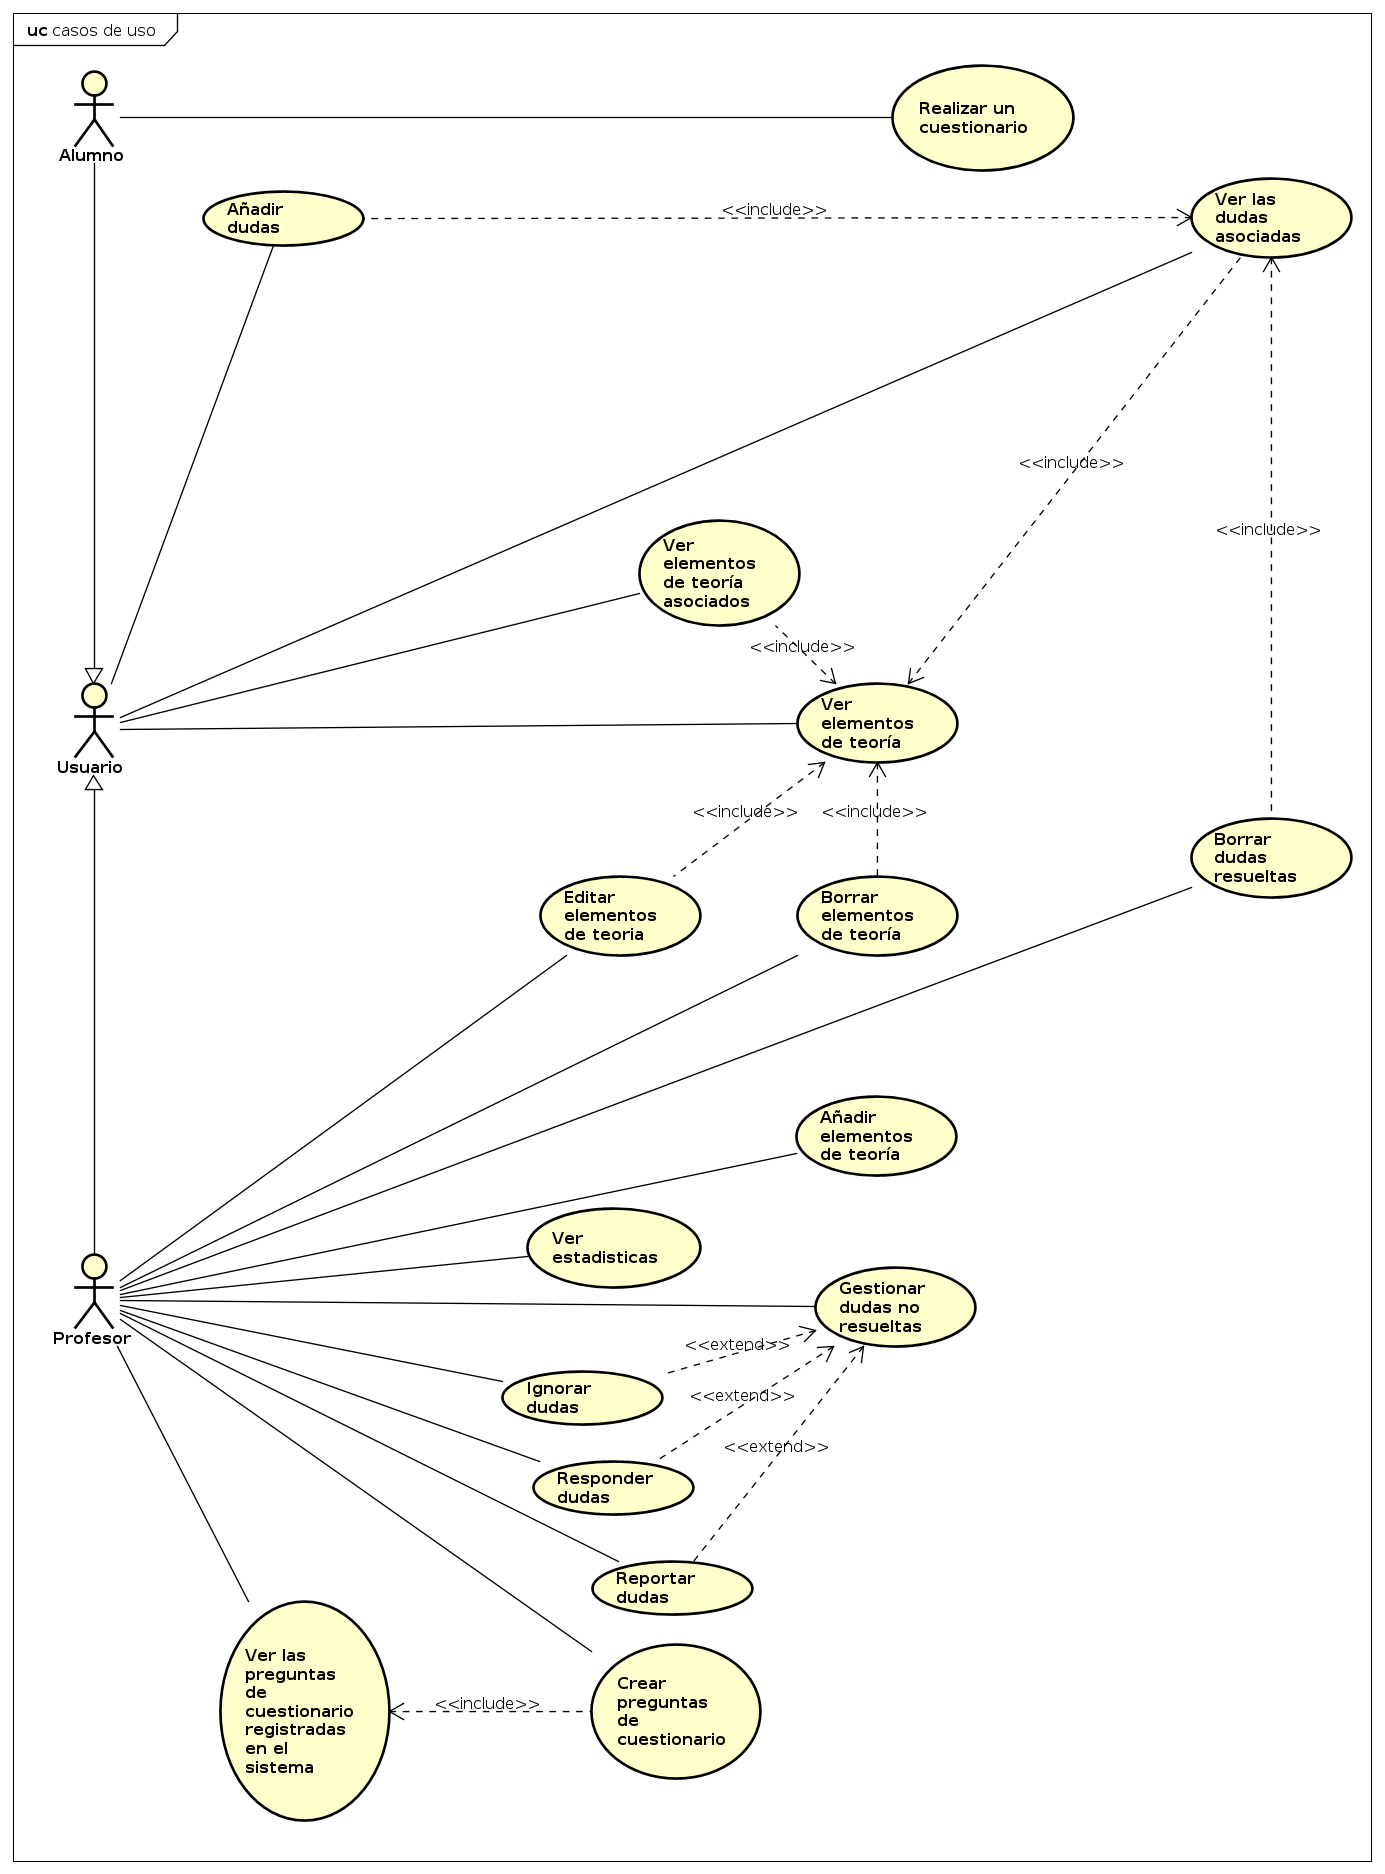
\includegraphics[scale=0.40]{img/astah/analisis/casos_de_uso/useCase00.png}
        \end{center}
        \caption{Diagrama de casos de uso}
    \end{figure}
    
    \newpage
    
    \subsubsection{Descripcion de los casos de
    uso}\label{descripcion-de-los-casos-de-uso}
    
    \vspace*{\fill}
    
    \begin{table}[H]
        \begin{center}
            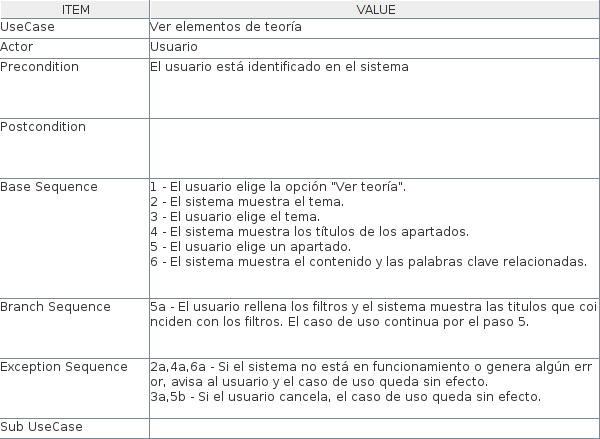
\includegraphics[width=\textwidth]{img/astah/analisis/casos_de_uso/useCase01.png}
        \end{center}
        \caption{Descripción del caso de uso Ver elementos de teoría}
    \end{table}
    
    \vspace*{\fill}
    
    \newpage
    
    \vspace*{\fill}
    
    \begin{table}[H]
        \begin{center}
            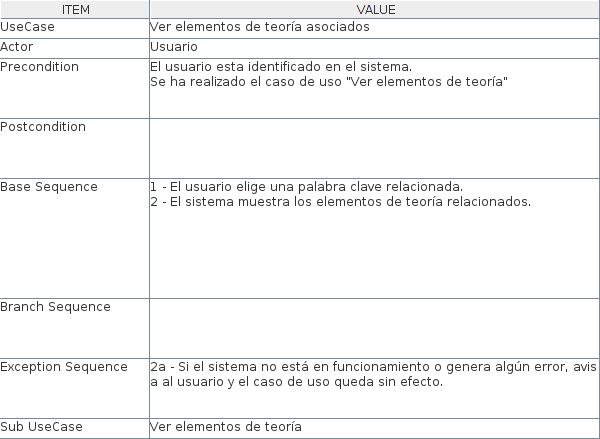
\includegraphics[width=\textwidth]{img/astah/analisis/casos_de_uso/useCase02.png}
        \end{center}
        \caption{Descripción del caso de uso Ver elementos de teoría asociados}
    \end{table}
    
    \vspace*{\fill}
    
    \newpage
    
    \vspace*{\fill}
    
    \begin{table}[H]
        \begin{center}
            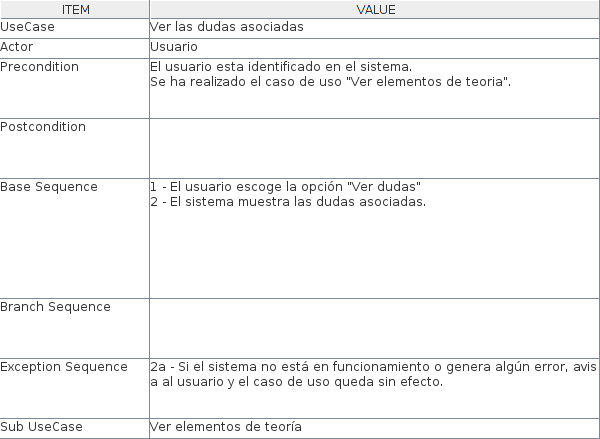
\includegraphics[width=\textwidth]{img/astah/analisis/casos_de_uso/useCase03.png}
        \end{center}
        \caption{Descripción del caso de uso Ver las dudas asociadas}
    \end{table}
    
    \vspace*{\fill}
    
    \newpage
    
    \vspace*{\fill}
    
    \begin{table}[H]
        \begin{center}
            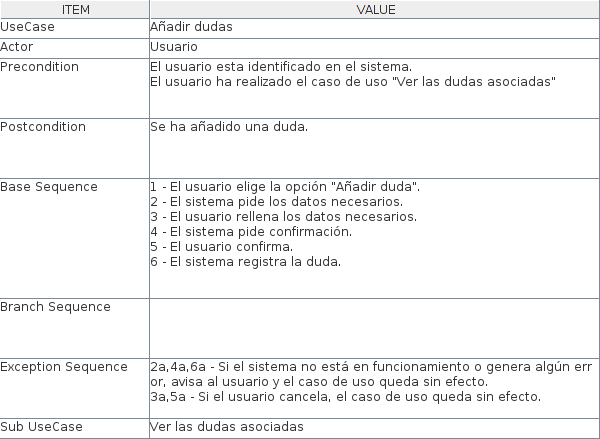
\includegraphics[width=\textwidth]{img/astah/analisis/casos_de_uso/useCase04.png}
        \end{center}
        \caption{Descripción del caso de uso Añadir dudas}
    \end{table}
    
    \vspace*{\fill}
    
    \newpage
    
    \vspace*{\fill}
    
    \begin{table}[H]
        \begin{center}
            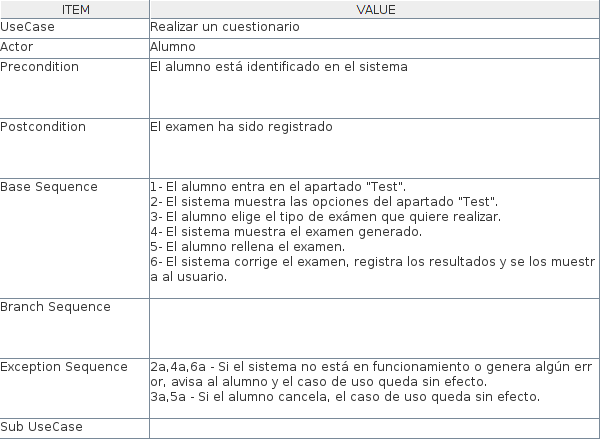
\includegraphics[width=\textwidth]{img/astah/analisis/casos_de_uso/useCase05.png}
        \end{center}
        \caption{Descripción del caso de uso Realizar un cuestionario}
    \end{table}
    
    \vspace*{\fill}
    
    \newpage
    
    \vspace*{\fill}
    
    \begin{table}[H]
        \begin{center}
            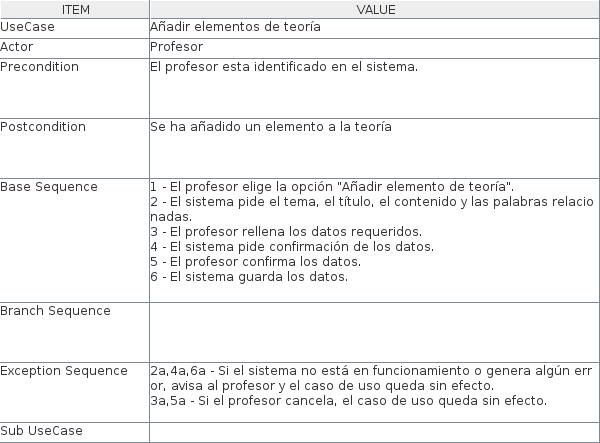
\includegraphics[width=\textwidth]{img/astah/analisis/casos_de_uso/useCase06.png}
        \end{center}
        \caption{Descripción del caso de uso Añadir elementos de teoría}
    \end{table}
    
    \vspace*{\fill}
    
    \newpage
    
    \vspace*{\fill}
    
    \begin{table}[H]
        \begin{center}
            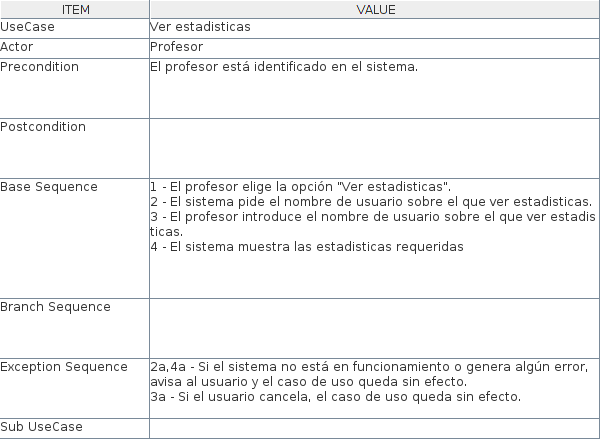
\includegraphics[width=\textwidth]{img/astah/analisis/casos_de_uso/useCase07.png}
        \end{center}
        \caption{Descripción del caso de uso Ver estadisticas}
    \end{table}
    
    \vspace*{\fill}
    
    \newpage
    
    \vspace*{\fill}
    
    \begin{table}[H]
        \begin{center}
            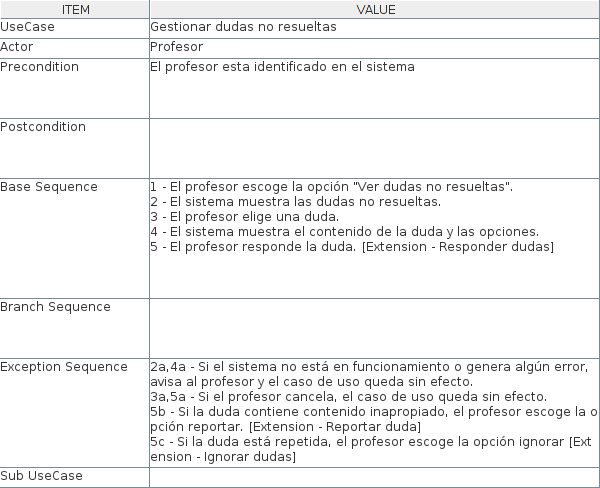
\includegraphics[width=\textwidth]{img/astah/analisis/casos_de_uso/useCase08.png}
        \end{center}
        \caption{Descripción del caso de uso Gestionar dudas no resueltas}
    \end{table}
    
    \vspace*{\fill}
    
    \newpage
    
    \vspace*{\fill}
    
    \begin{table}[H]
        \begin{center}
            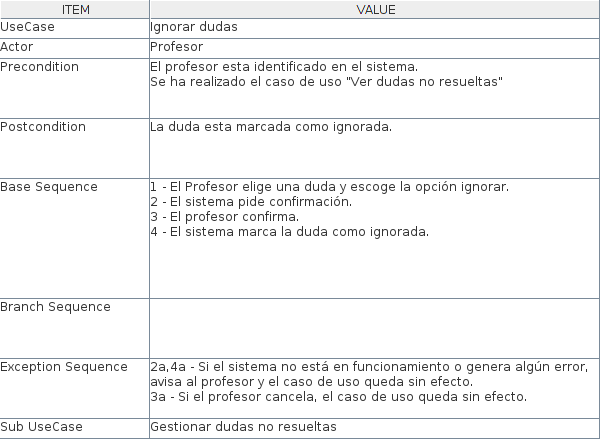
\includegraphics[width=\textwidth]{img/astah/analisis/casos_de_uso/useCase09.png}
        \end{center}
        \caption{Descripción del caso de uso Ignorar dudas}
    \end{table}
    
    \vspace*{\fill}
    
    \newpage
    
    \vspace*{\fill}
    
    \begin{table}[H]
        \begin{center}
            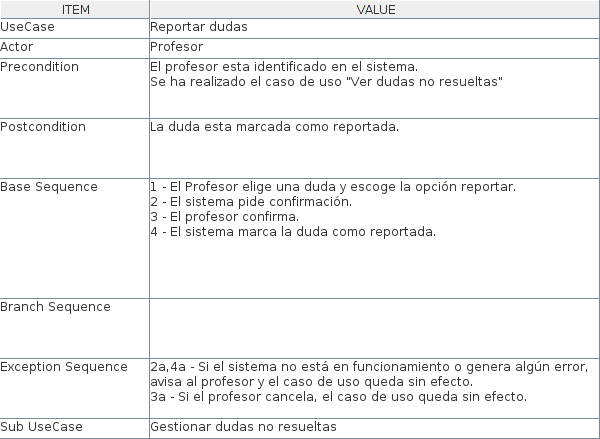
\includegraphics[width=\textwidth]{img/astah/analisis/casos_de_uso/useCase10.png}
        \end{center}
        \caption{Descripción del caso de uso Reportar dudas}
    \end{table}
    
    \vspace*{\fill}
    
    \newpage
    
    \vspace*{\fill}
    
    \begin{table}[H]
        \begin{center}
            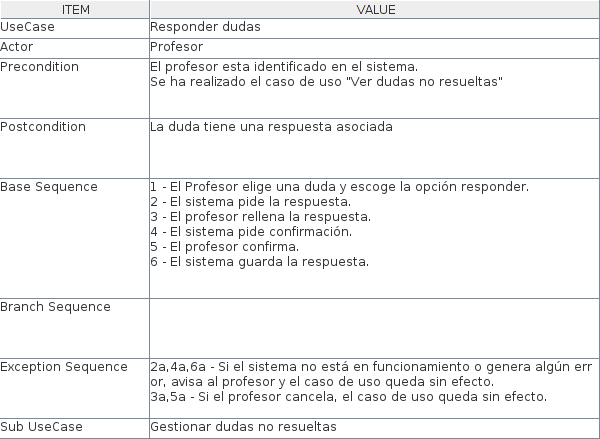
\includegraphics[width=\textwidth]{img/astah/analisis/casos_de_uso/useCase11.png}
        \end{center}
        \caption{Descripción del caso de uso Responder dudas}
    \end{table}
    
    \vspace*{\fill}
    
    \newpage
    
    \vspace*{\fill}
    
    \begin{table}[H]
        \begin{center}
            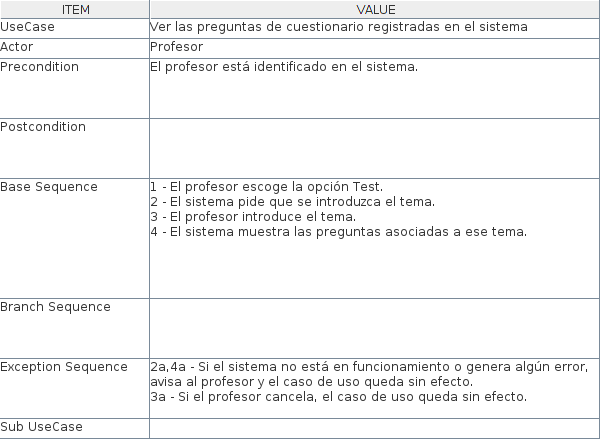
\includegraphics[width=\textwidth]{img/astah/analisis/casos_de_uso/useCase12.png}
        \end{center}
        \caption{Descripción del caso de uso Ver las preguntas de cuestionario registradas en el sistema}
    \end{table}
    
    \vspace*{\fill}
    
    \newpage
    
    \vspace*{\fill}
    
    \begin{table}[H]
        \begin{center}
            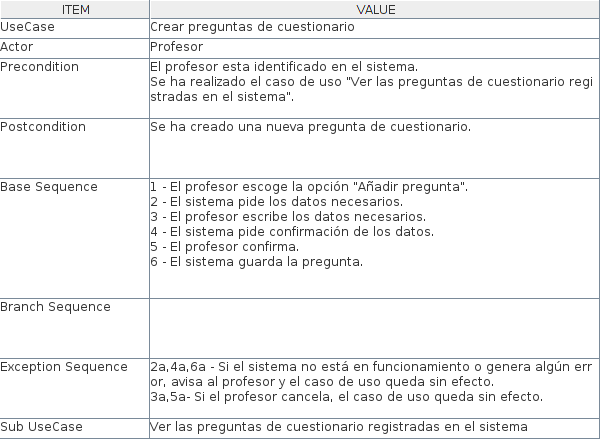
\includegraphics[width=\textwidth]{img/astah/analisis/casos_de_uso/useCase13.png}
        \end{center}
        \caption{Descripción del caso de uso Crear preguntas de cuestionario}
    \end{table}
    
    \vspace*{\fill}
    
    \newpage
    
    \vspace*{\fill}
    
    \begin{table}[H]
        \begin{center}
            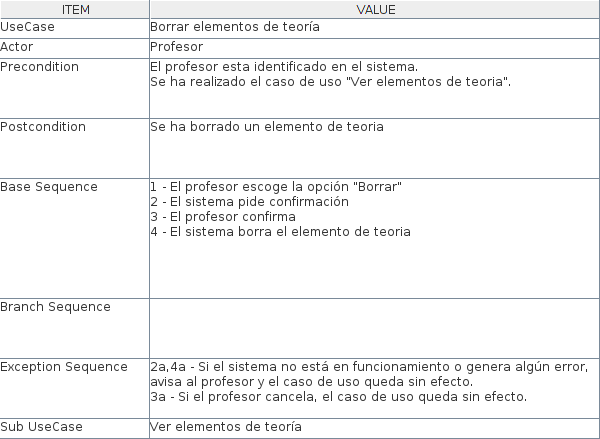
\includegraphics[width=\textwidth]{img/astah/analisis/casos_de_uso/useCase14.png}
        \end{center}
        \caption{Descripción del caso de uso Borrar elementos de teoría}
    \end{table}
    
    \vspace*{\fill}
    
    \newpage
    
    \vspace*{\fill}
    
    \begin{table}[H]
        \begin{center}
            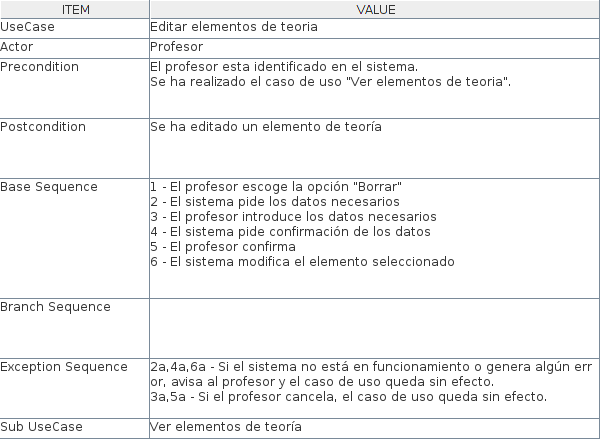
\includegraphics[width=\textwidth]{img/astah/analisis/casos_de_uso/useCase15.png}
        \end{center}
        \caption{Descripción del caso de uso Editar elementos de teoria}
    \end{table}
    
    \vspace*{\fill}
    
    \newpage
    
    \vspace*{\fill}
    
    \begin{table}[H]
        \begin{center}
            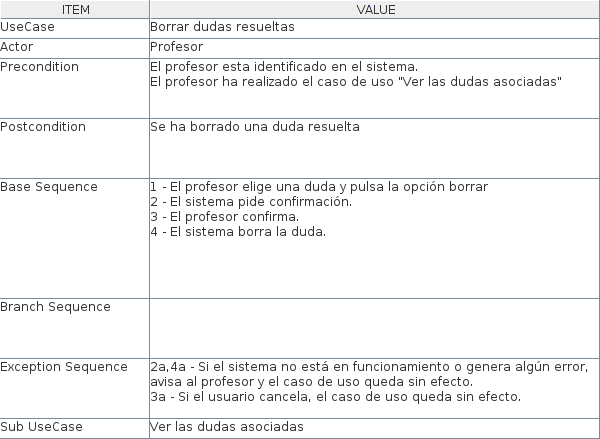
\includegraphics[width=\textwidth]{img/astah/analisis/casos_de_uso/useCase16.png}
        \end{center}
        \caption{Descripción del caso de uso Borrar dudas resueltas}
    \end{table}
    
    \vspace*{\fill} \newpage
    
    \subsection{Modelo de dominio}\label{modelo-de-dominio}
    
    \vspace*{\fill}
    
    \begin{figure}[H]
        \begin{center}
            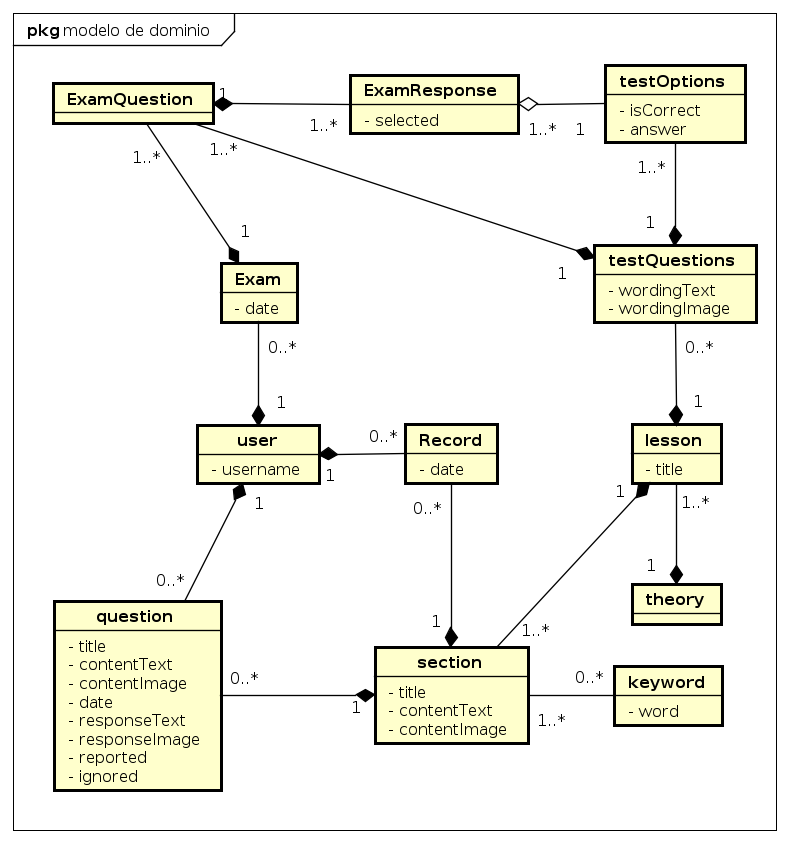
\includegraphics[width=\textwidth]{img/astah/analisis/dominio/modelo.png}
        \end{center}
        \caption{Modelo de dominio}
    \end{figure}
    
    \vspace*{\fill}
    
    \newpage
    
    \section{Diseño}\label{diseuxf1o}
    
    \subsection{Diseño de la base de
    datos}\label{diseuxf1o-de-la-base-de-datos}
    
    \newpage
    
    \subsection{Despliegue}\label{despliegue}
    
    \vspace*{\fill}
    
    \begin{figure}[H]
        \begin{center}
            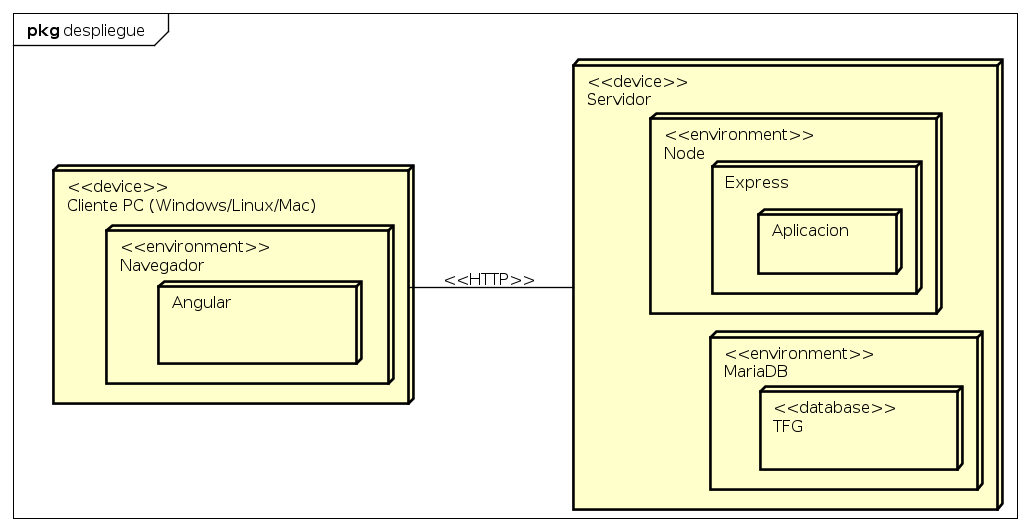
\includegraphics[width=\textwidth]{img/astah/disenio/despliegue/deployment.png}
        \end{center}
        \caption{Diagrama de despliegue}
    \end{figure}
    
    \vspace*{\fill} \newpage
    
    \subsection{Arquitectura del sistema}\label{arquitectura-del-sistema}
    
    \subsubsection{Front-end}\label{front-end}
    
    \subsubsection{Back-end}\label{back-end}
    
    \subsection{Diagrama de clases}\label{diagrama-de-clases}
    
    \subsection{Diagramas de secuencia}\label{diagramas-de-secuencia}
    
    \chapter{ Conclusiones }
    
    Conclusiones
    
    \section{Trabajo futuro}\label{trabajo-futuro}
    
    Como mejorar la aplicacion
    
    \appendix
    
    \chapter{ Manual de despliegue }
    
    Para desplegar esta aplicación necesitamos:
    
    \begin{itemize}
    \item
      Un ordenador con un sistema operativo basado en UNIX con node y npm
      instalados
    \item
      Conexión a Internet(para descargar dependencias)
    \item
      El código fuente de la aplicación.
    
      Aunque se entrega en el CD, esta disponible en
      https://github.com/Raikuro/TFG
    \end{itemize}
    
    Pasos a realizar para desplegar:
    
    \begin{enumerate}
    \def\labelenumi{\arabic{enumi}.}
    \tightlist
    \item
      \textbf{Modificar los ficheros de configuración:}
    \end{enumerate}
    
    Para entenderlos ficheros de configuración se explica la máquina en la
    que está actualmente desplegada la aplicación.
    
    La máquina es accesible mediante la dirección
    `http://virtual.lab.inf.uva.es' en el puerto 20052. Debido a la
    configuración interna de la máquina, redirige el puerto interno 80 al
    puerto externo 20052 y el puerto 3000 al 20053.
    
    Los ficheros que es necesario modificar son los siguientes:
    
    \begin{itemize}
    \item
      backend/config/client.js:
    
    \begin{verbatim}
    const IP = 'http://virtual.lab.inf.uva.es'
    const PORT = 20052 
    exports.ADDRESS = IP + ':' + PORT
    \end{verbatim}
    
      Es necesario cambiar las constantes IP y PORT por la IP y el puerto
      desde el cual será accesible nuestro frontend.
    \item
      frontend/.angular-cli.json:
    
    \begin{verbatim}
    ...
    "defaults": {
      "styleExt": "css",
    "component": {},
    "serve": {
      "host": "10.0.20.5",
      "port": 80
    }
      }
    ...
    \end{verbatim}
    
      Es necesario cambiar los parámetros host y port por la IP y el puerto
      interno en el que desplegaremos nuestro frontend
    \item
      frontend/src/app/config/server.ts
    
    \begin{verbatim}
    const IP = "http://virtual.lab.inf.uva.es";
    const PORT = 20053;
    export const ADDRESS = IP + ":" + PORT
    \end{verbatim}
    
      Es necesario cambiar las constantes IP y PORT por la IP y el puerto
      desde el cual será accesible nuestro backend
    \end{itemize}
    
    \begin{enumerate}
    \def\labelenumi{\arabic{enumi}.}
    \setcounter{enumi}{1}
    \tightlist
    \item
      \textbf{Instalar las dependencias:}
    \end{enumerate}
    
    Se ejecutarán los siguientes comandos desde la raiz del CD
    
    \begin{verbatim}
    cd backend
    npm install
    cd frontend
    npm install
    \end{verbatim}
    
    \begin{enumerate}
    \def\labelenumi{\arabic{enumi}.}
    \setcounter{enumi}{2}
    \tightlist
    \item
      \textbf{Desplegar:}
    \end{enumerate}
    
    Se ejecutarán los siguientes comandos desde la raiz del CD para
    desplegar el frontend
    
    \begin{verbatim}
    cd frontend
    npm start
    \end{verbatim}
    
    Se ejecutarán los siguientes comandos desde la raiz del CD para
    desplegar el backend
    
    \begin{verbatim}
    cd backend
    npm start
    \end{verbatim}
    
    \chapter{Manual de usuario}\label{manual-de-usuario}
    
    \chapter{Contenido del CD-ROM}\label{contenido-del-cd-rom}
    
    \addcontentsline{toc}{chapter}{Bibliografía}
    
    \nocite{*} \printbibliography

    \cleardoublepage
    %\renewcommand\bibname{Referencias Web}

    %\begin{thebibliography}{X}
    %    \bibitem{ref1} \textit{Ejemplo}, \\
    %    \textsc{ejemplo.com}.
    %    \\Recuperado a tal fecha, \\de \href{http://ejemplo.com}
    %\end{thebibliography}
\end{document}